\begin{figure}
\centering
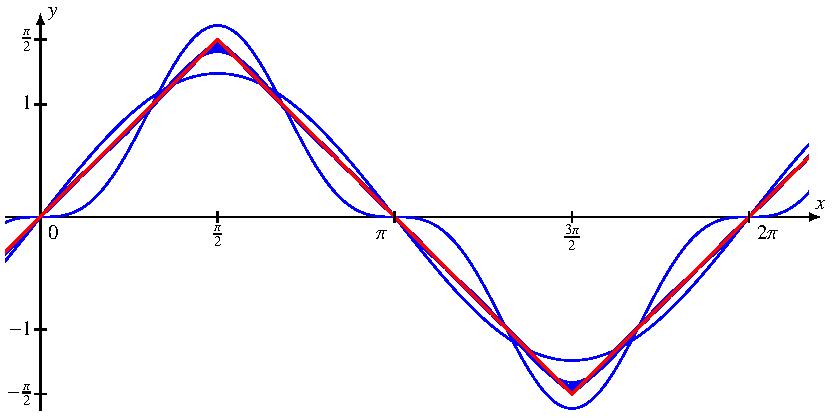
\includegraphics{chapters/010-skalarprodukt/images/fourierdreieck.pdf}
\caption{Die 
Reihe~\ref{buch:skalarprodukt:sobolevraum:eqn:fourierdreieck}
mit beliebig oft stetig differenzierbaren Partialsummen konvergiert
gleichmässig gegen die stetige Dreiecksfunktion, aber die Grenzfunktion
ist nicht mehr überall differenzierbar.
\label{buch:skalarprodukt:sobolevraum:fig:fourierdreieck}}
\end{figure}
